\chapter{Proposed Method}

Aim of this project is to develop a testbed that aids in the development of reinforcement learning algorithms for robot manipulation tasks. The test-bed should be able to scale the training speed with computational power by running multiple simulations in parallel. It should use standard frameworks that support training distributed RL algorithms. It should also have a flexible architecture that allows other researchers to add new types of robot manipulation task and test new RL algorithms.

\begin{figure}[H]
	\centering
	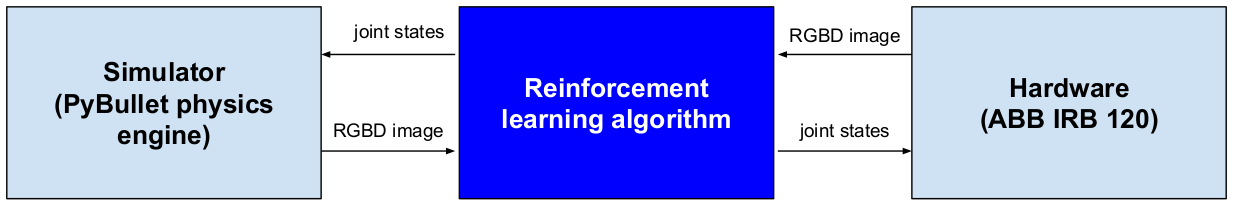
\includegraphics[scale=0.3]{overall-block-diagram}
	\caption{Testbed methodology block diagram}
	\label{fig:simulation-arch}
\end{figure}

Robot manipulation tasks can be evaluated on both simulation environment and real robot. The testbed will provide inbuilt support for simulated and real ABB IRB 120 robot. For training the RL algorithm, simulated environment will be used. This allows scaling training speed with computational power by running multiple instances of simulator in parallel. Policies learned from simulator can be evaluated on real ABB IRB 120 robot. A RGB-D camera will be mounted on the end-effector of robot. The only input to RL algorithm will be the RGB image with depth map from RGB-D camera. The RL algorithm will take this input and output the desired joint states of robot in order to achieve a particular task. Simulator / hardware will take the desired joint states as input and apply torques on joints to achieve desire joint state

\section {Simulation setup}
All reinforcement learning agents are first trained in a simulated environment. In this project the simulated environment is created using Bullet Physics Simulator.

\subsection{Setup}
\begin{figure}[H]
	\centering
	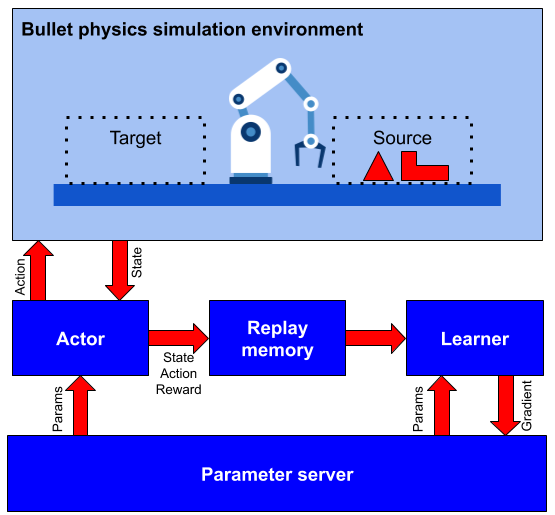
\includegraphics[scale=0.5]{simulation-arch}
	\caption{Standard simulation architecture}
	\label{fig:simulation-arch}
\end{figure}

To reduce training time, agent training via simulation is parallelized and distributed similar to GORILA architecture \cite{gorila}. In this project we use Ray RLLib \cite{rllib} which provides abstractions for distributed reinforcement learning.

\subsubsection{Environment}
Simulation environment is developed using Bullet Physics simulator python module. Environment will be setup for a specific task like table clearing or stacking of objects. Environment will accept actions from specific task which must be in specific format according to action space of environment. When environment receives an action, it will apply the action to simulated environment using PyBullet APIs. After action is completed, the environment will record the state according to state space of environment and calculate the reward according to task setup of environment. Environment returns state and reward after action is applied.

\subsubsection{PyBullet Simulator}
PyBullet is a python module for Bullet Physics C SDK used for physics simulation in robotics, games, visual effects and machine learning, with a focus on sim-to-real transfer \cite{pybullet}. PyBullet can load visual, physical and other properties of a body from URDF, SDF and Mujoco formats. If required, 3D mesh of bodies can be loaded directly using PyBullet APIs. For simulating robots, PyBullet supports forward and inverse kinematics, collision detection, coordinate transformations, forward dynamics simulation, inverse dynamics computation, joint state position, velocity and force/torque control.

PyBullet supports rendering using CPU renderer and OpenGL renderer. Visualization can be optionally turned off in PyBullet. With visualization disabled, PyBullet uses CPU renderer for rendering images captured by camera API. This is especially useful in reinforcement learning where we want to collect data from simulated environment as fast as possible.

\subsubsection{Actor}
Actor is responsible for reading policy from the parameter server and execute actions is the simulation environment and save the action, returned state, returned reward in experience replay memory. When an actor is started, it will create a new simulation environment process. 
\begin{itemize}
	\item Start new simulation environment process
	\item Begin new episode
	\item Read policy ($\pi(a_t|s_t)$) and environment state ($s_t$). Evaluate and select action $a_t$ for state $s_t$ by evaluating policy $\pi(a_t|s_t)$. Execute the action $a_t$ on simulation environment environment and read the returned reward $r_t$ and new state of environment $s_{t+1}$. Save $[a_t, s_t, r_t, s_{t+1}]$ to replay buffer
	\item End episode when simulation environment terminates an episode
\end{itemize}

\subsubsection{Replay buffer}
Replay buffer stores the trajectory of episodes. Trajectory of an episode is a list of $[a_t, s_t, r_t, s_{t+1}]$. Since multiple actor process are supposed to add observations to replay buffer, replay buffer is usually a distributed database accessible by actor processes. 

\subsubsection{Learner}
Learner reads the episode trajectories stored in replay buffer and optimize the policy stored in parameter server to maximize rewards. Learner process is specific to a reinforcement learning algorithm. Eg:- DDPG, PPO. Learner process uses deep learning frameworks like tensorflow or pytorch to model the policy, calculate the gradients for loss functions and do other computations.

\subsubsection{Parameter server}
Parameter server stores the policy. It is accessible by both actor and learner and also accepts gradient from learner and apply the gradient to update the policy represented by parameter server.


\section{Hardware setup}
\begin{figure}[H]
	\centering
	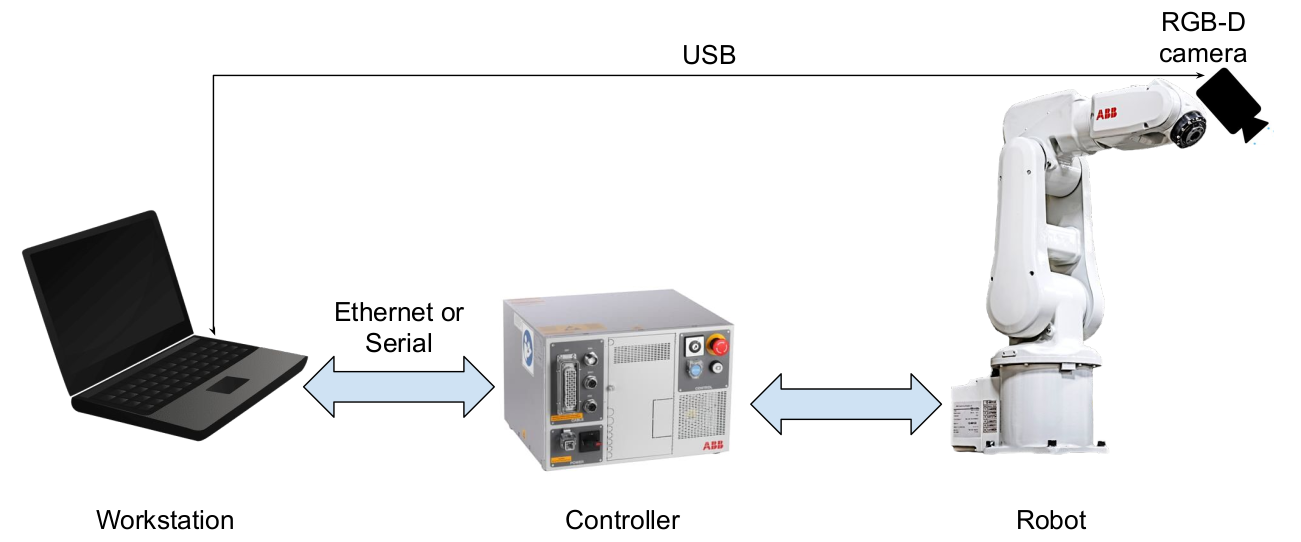
\includegraphics[scale=0.3]{hardware-setup}
	\caption{Hardware setup architecture}
	\label{fig:hardware-arch}
\end{figure}

Policies learned from simulator will be evaluated on ABB IRB 120 robot. Depth camera mounted on endeffector will provide visual feedback. Camera will be directly connected to computer. Program running in the computer will directly connect with via serial or ethernet port in robot controller. RAPID program running on robot will read actions send from computer, execute it and send feedback to computer.

For ethernet connectivity, ABB robot studio license requires PC interface capability. This capability is not available in license available at robotics lab in CET. Also we were unable to establish bi-directional connection via virtual serial port between workstation and simulated ABB robot controller. Trying to establish bidirectional serial connection was also crashing the simulated ABB robot controller. So to keep it safe, we didn't tried to connect workstation and real ABB robot controller via serial port. This two limitations prevented us from connecting workstation with real robot controller and plan to integrate testbed with ABB IRB 120 hardware was dropped.

\section{Reinforcement learning algorithm}
Reinforcement learning algorithm takes RGB-D image as input and provides joint state as output. The testbed will have prebuilt support for following baseline RL algorithm.

\subsection{Proximal Policy Optimization (PPO)}
PPO is an on policy, stochastic and policy gradient based reinforcement learning method \cite{ppo}. The objective function of PPO is 

\begin{equation}
L^{CLIP} (\theta) = \hat{E}_t \left[ min(r_t(\theta) \hat{A}_t, clip(r_t(\theta), 1 - \epsilon, 1 + \epsilon) \hat{A}_t) \right]
\end{equation}

Where
\begin{itemize}
	\item $\theta$ is the policy parameter
	\item $\hat{E}_t$ denotes the empirical expectation over timesteps
	\item $r_t$ is the ratio of probability under the new and old policies, respectively
	\item $\hat{A}_t$ is the estimated advantage at time $t$
	\item $\epsilon$ is a hyperparameter, usually 0.1 or 0.2
\end{itemize}

\subsubsection{Architecture}
PPO requires two neural networks, value network to calculate advantage of taking an action and policy network for predicting mean and variance of an action to maximize reward at a given state. We use 3 layer CNN for extracting features from image of gripper camera. The input image shape is $84 \times 84 \times 4$. Fourth channel is depth value. The value network and policy network can share this 3 layer CNN for feature extraction. But since loss functions of value network and policy network are different, sharing the CNN layers might optimize the CNN layers for either value or policy network. This can be fixed by scaling the loss functions of value and policy network to same scale.

\begin{figure}[H]
	\centering
	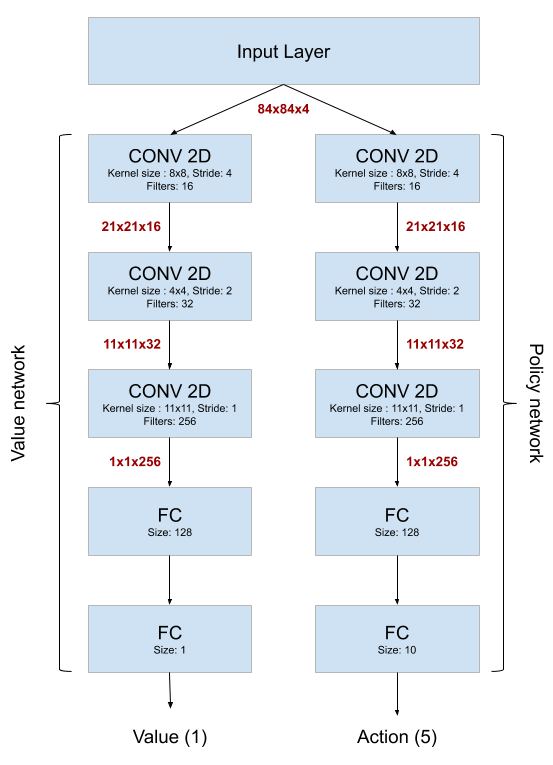
\includegraphics[scale=0.5]{ppo-arch}
	\caption{PPO network architecture}
\end{figure}